\section{多资产协同搜索（15 种组合）}\label{sec:multi}

\subsection{设定}

在单船评估的基础上，考虑“多艘同配置船 + 多台 AUV”同时搜索：

\begin{itemize}[leftmargin=1.8em,itemsep=0pt]
\item 每艘船 = 母船同款 M4 配置（雷达 + 深水侧扫 + 深水多波束 + ROV）；
\item \textbf{$t=0$ 时只有母船}在失事点上方；增援船与 AUV 在 \textbf{3 h} 后到位：
      增援船从出发岛出发（转场约 0.5--1 h），AUV 由母船投放；
\item 组合：船数 $2$--$4$（含母船）$\times$ AUV 数 $0$--$4$，共 $3\times5=15$ 种；
\item 成本 = 母船 M4 基线 182 + $70\times(\text{船数}-1)$ + $57\times\text{AUV 数}$（万美元）。
\end{itemize}

\subsection{结果}

\begin{table}[H]
\centering\small
\caption{15 种多船/多 AUV 组合的 72 h 成功率（完整表见数据文件）}
\label{tab:multi}
\begin{tabular}{@{}lccccc@{}}
\toprule
船数 $\backslash$ AUV 数 & 0 & 1 & 2 & 3 & 4\\
\midrule
2 艘（252--480 万） & 96.6\% & 98.3\% & 98.9\% & 99.3\% & 99.4\%\\
3 艘（322--550 万） & 98.4\% & 99.2\% & 99.5\% & 99.6\% & 99.7\%\\
4 艘（392--620 万） & 99.2\% & 99.5\% & 99.7\% & 99.8\% & 99.9\%\\
\bottomrule
\end{tabular}
\end{table}

\begin{figure}[H]
\centering
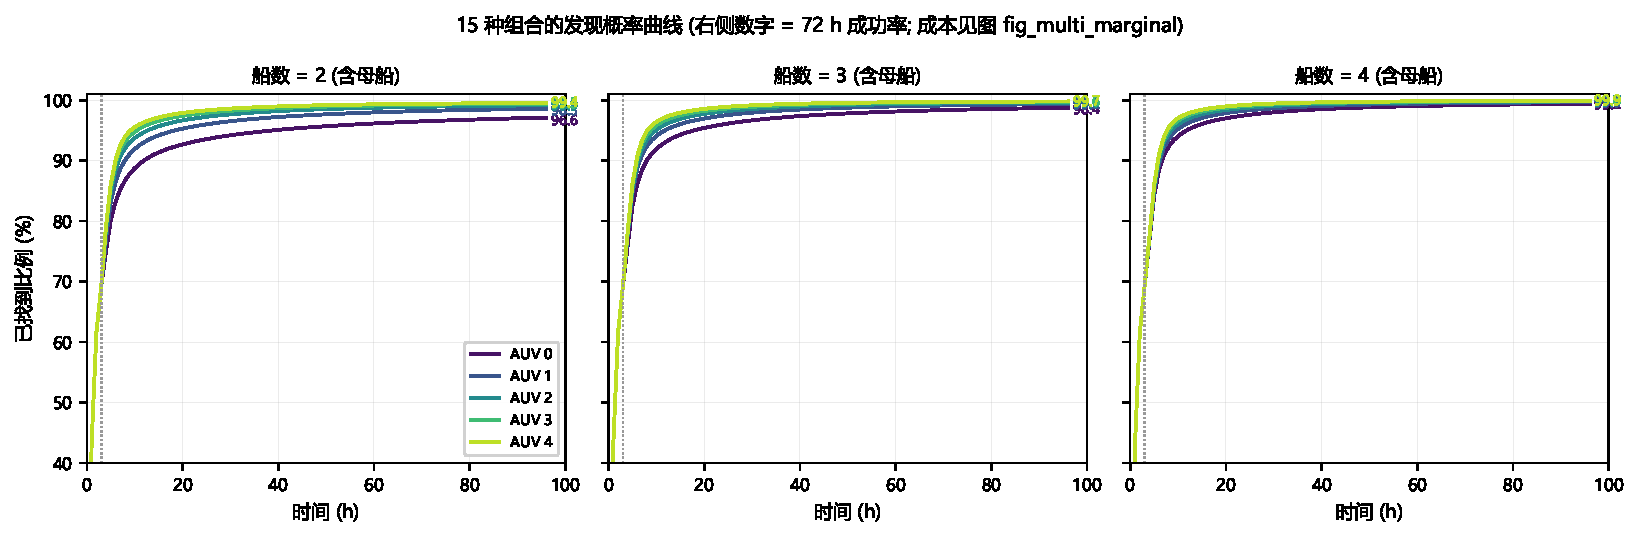
\includegraphics[width=0.80\textwidth]{fig_multi_curves}
\caption{15 种组合的 $P(t)$ 曲线（按船数分组，右侧数字为 $P_{72}$）。}
\label{fig:multi-curves}
\end{figure}



\subsection{协调规则与重复扫描}\label{sec:multi-beta}

多资产容易“扎堆”搜索同一片高概率区域。我们用两条规则控制：
小时内认领（同格同小时只派一次）与重复扫描惩罚 $\beta$。
\tabref{tab:beta} 给出“2 艘船”场景下 $\beta$ 的调优结果：$\beta=1$ 时
$P_{72}$ 只降 0.6 个百分点，跨小时重复扫描率从 35.6\% 降到 27.5\%；
同小时重复率在所有设置下严格为 0。

\begin{table}[H]
\centering\small
\caption{重复扫描惩罚 $\beta$ 的调优（2 艘船场景）}
\label{tab:beta}
\begin{tabular}{@{}lrrrrrr@{}}
\toprule
$\beta$ & 0 & 0.2 & 0.5 & 1.0（采用） & 2.0 & 5.0\\
\midrule
$P_{72}$ & 97.2\% & 97.2\% & 97.0\% & 96.6\% & 95.6\% & 91.8\%\\
跨小时重复率 & 35.6\% & 32.2\% & 29.9\% & 27.5\% & 24.8\% & 20.8\%\\
\bottomrule
\end{tabular}
\end{table}



\begin{figure}[H]
\centering
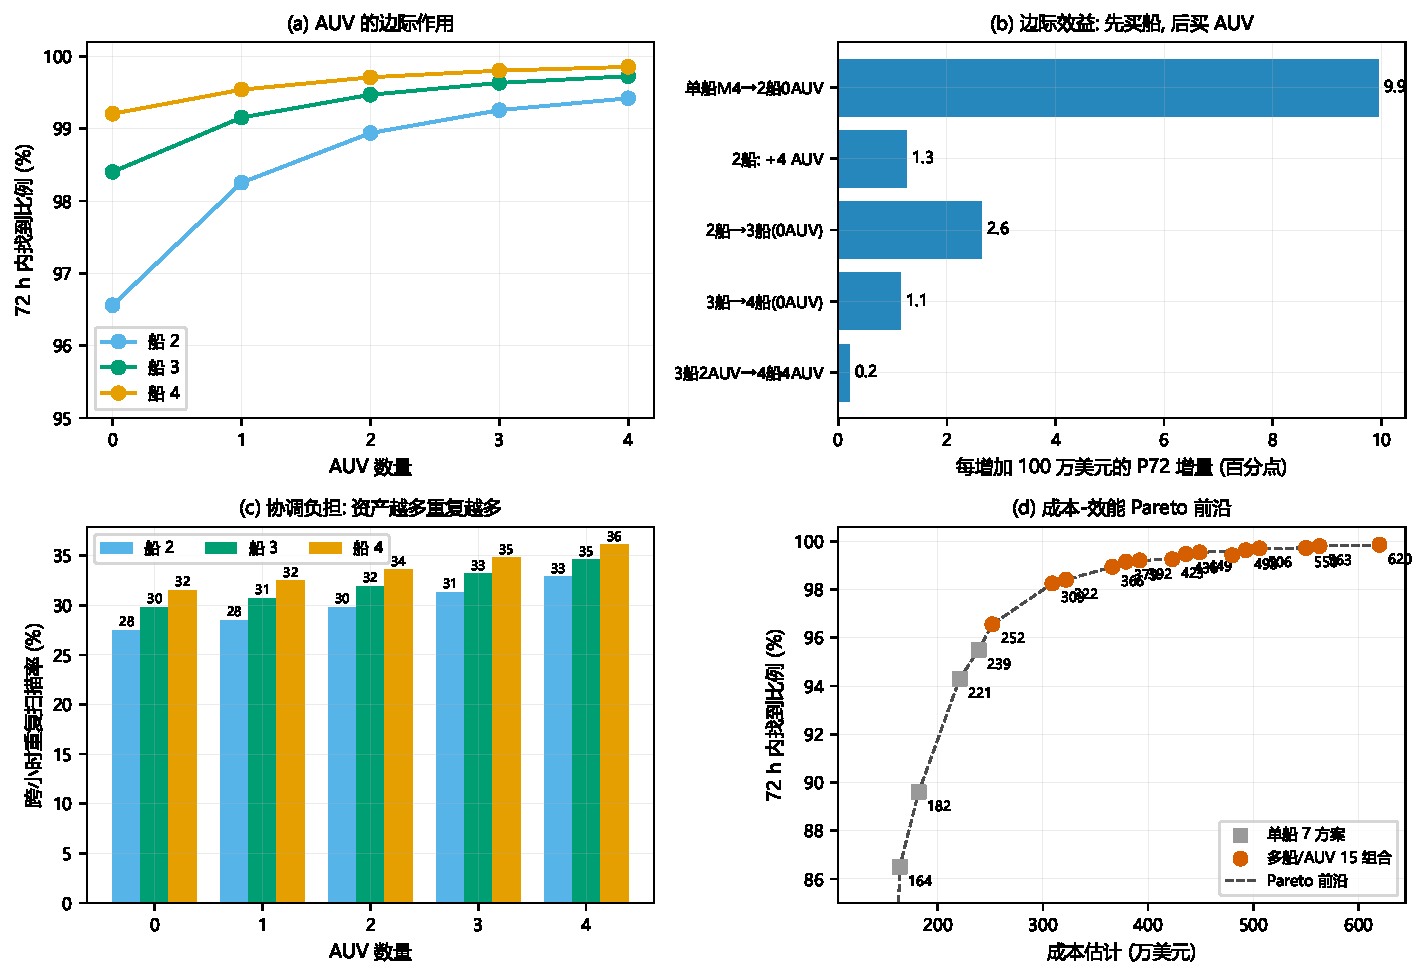
\includegraphics[width=0.76\textwidth]{fig_multi_marginal}
\caption{多资产分析的四个视角：(a) AUV 的边际作用；(b) 每 100 万美元带来的
$P_{72}$ 增量（“单船$\to$2 船”为 9.9 个百分点/百万，远高于加 AUV 的 1.3）；
(c) 协调负担（资产越多重复扫描率越高）；(d) 成本–效能 Pareto 前沿。}
\label{fig:marginal}
\end{figure}

\paragraph{路径规划示例.} \figref{fig:multi-plan} 给出“3 船 + 2 AUV”在示例案例中的
实际搜索航迹与网格被搜索次数。可以看到：搜索努力集中在预测云的高概率区，
并沿漂移方向向外扩展；增援船从出发点（右下角外）进入后接替母船覆盖新区域。

\begin{figure}[H]
\centering
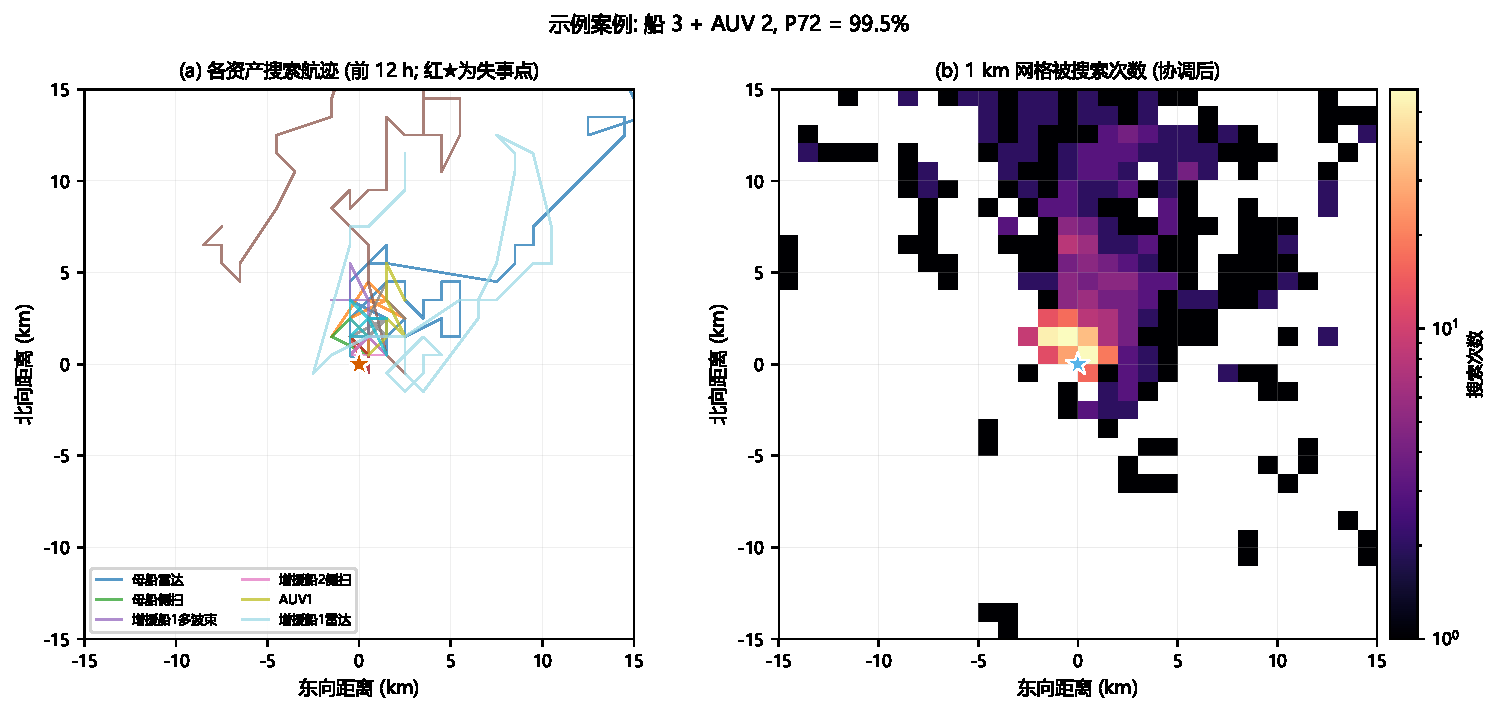
\includegraphics[width=0.86\textwidth]{fig_multi_plan}
\caption{示例案例（3 船 + 2 AUV）。(a) 前 12 h 各资产搜索航迹；(b) 1 km 网格被搜索
次数的对数热图——集中的高概率区被多轮补扫，外围较新区域只扫描一次。}
\label{fig:multi-plan}
\end{figure}

\paragraph{增援到位时间.} 将“3 h 到位”作为基准，做 0/3/6/12 h 敏感性
（\figref{fig:multi-delay}）：最简增援方案（2 船）对到位时间最敏感，每推迟 3 h
$P_{72}$ 降约 0.6--0.9 个百分点；冗余度高的方案（4 船+4 AUV）几乎不敏感。

\begin{figure}[H]
\centering
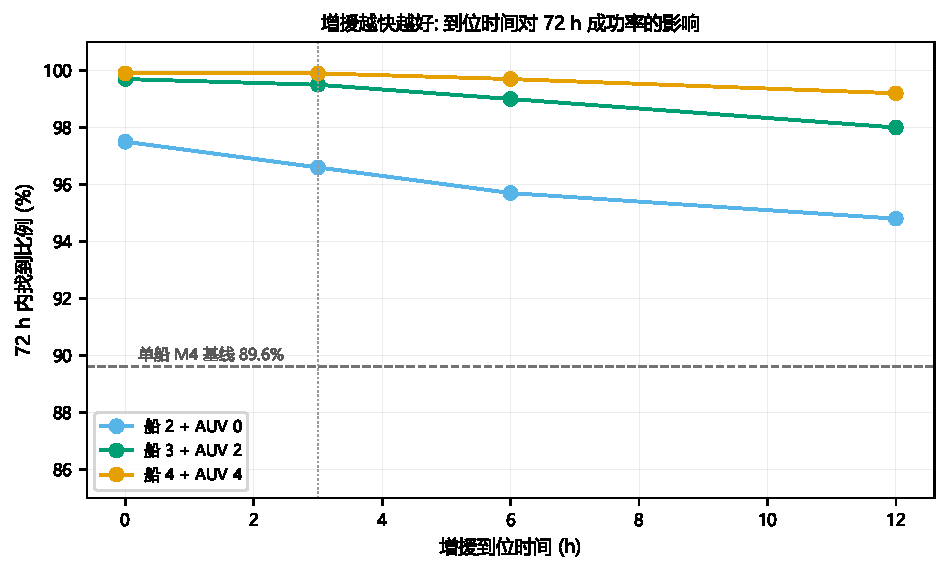
\includegraphics[width=0.62\textwidth]{fig_multi_delay}
\caption{增援到位时间对 $P_{72}$ 的影响（虚线为单船 M4 基线 89.6\%）。}
\label{fig:multi-delay}
\end{figure}

\subsection{多资产结论}

\begin{enumerate}[leftmargin=1.8em,itemsep=0pt]
\item \textbf{“加 1 艘船”是全部选项里性价比最高的一步}：$P_{72}$ 从 89.6\% 到 96.6\%
      （+7.0 个百分点），成本从 182 万到 252 万（每百万 9.9 个百分点），
      远高于“加 4 台 AUV”的 1.3；
\item \textbf{“2 船 + 2 AUV”（366 万，98.9\%）是高保障方案的甜点}；
\item \textbf{4 船 + 4 AUV（620 万）只有 99.9\%}，边际收益接近零——继续堆装备不如
      把资源投在“缩短响应时间”与“提高预报精度”上；
\item 协调规则（认领 + 惩罚）使同小时重复率严格为 0，跨小时重复率控制在 27\%--36\%，
      这是多资产方案能“加船就有用”的前提。
\end{enumerate}
